\section{IPFS} 

It is well known that the Ethereum blockchain is not suited for saving data. You just need to know that for hypothetically uploading a file on Ethereum, you would have to pay about 2\$ per kilobyte. 
\\
For these reasons, we adopted the InterPlanetary File System (IPFS) protocol in the homonymous peer-to-peer network to store all the information that is not involved in VAT management. Specifically, for security purposes, all the data used to make payments between the clients are exclusively stored in the Ethereum blockchain. All the remaining data, such as not sensitive clients' data, products' data, orders' data, are stored into IPFS since it is a free and distributed technology born with the aim of sharing every kind of content.

\subsection{Architecture overview}

To establish a connection to the IPFS network we developed a small package that is responsible for hiding the IPFS connection implementation (\texttt{ipfs-mini} API\glo). The available interface contains two methods: one for adding new data into the blockchain, and the other one for retrieving them starting from the IPFS content identifier (CID).
\begin{figure}[h]
	\centering
	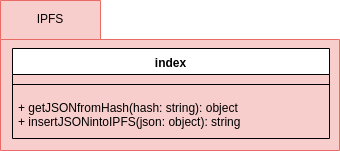
\includegraphics[scale=0.6]{res/images/IPFS.png}
	\caption{Class diagram of the IPFS package}
\end{figure}
\subsection{Methods}
The package provides the following methods:
\begin{itemize}
	\item \textbf{getJSONfromHash}: it uses the \texttt{ipfs-mini} API to retreive the JSON object corresponding to the passed IPFS CID;
	\item \textbf{insertJSONintoIPFS}: it uses the \texttt{ipfs-mini} API to upload the JSON passed to the function, then returns the IPFS CID.
\end{itemize}

\subsection{How to extend with new features}
The two functions we are providing lets the user save any kind of information in the JSON format. Since the aim of this package is to interact with IPFS, the possible changes that could be done are:
\begin{itemize}
	\item the implementation of the addition of data saved in formats different from JSON. In this case, we suggest to look at the documentation of the package \texttt{ipfs\_mini}, which API is actually used to retrieve data since it offers a large variety of functions;
	\item the change of the API package. If it is appropriate to use another package in order to carry out the writings and readings from IPFS, the developer must be sure not to alter the signature and the behaviour of the already offered functions.
\end{itemize}